% ****** Start of file aipsamp.tex ******
%
%   This file is part of the AIP files in the AIP distribution for REVTeX 4.
%   Version 4.1 of REVTeX, October 2009
%
%   Copyright (c) 2009 American Institute of Physics.
%
%   See the AIP README file for restrictions and more information.
%
% TeX'ing this file requires that you have AMS-LaTeX 2.0 installed
% as well as the rest of the prerequisites for REVTeX 4.1
%
% It also requires running BibTeX. The commands are as follows:
%
%  1)  latex  aipsamp
%  2)  bibtex aipsamp
%  3)  latex  aipsamp
%  4)  latex  aipsamp
%
% Use this file as a source of example code for your aip document.
% Use the file aiptemplate.tex as a template for your document.
\documentclass[%
 aip,
 jmp,%
 amsmath,amssymb,
%preprint,%
 reprint,%
%author-year,%
%author-numerical,%
]{revtex4-1}
\usepackage{textcomp}
\usepackage{graphicx}% Include figure files
\usepackage{dcolumn}% Align table columns on decimal point
\usepackage{bm}% bold math
%\usepackage[mathlines]{lineno}% Enable numbering of text and display math
%\linenumbers\relax % Commence numbering lines

\usepackage{enumerate}
\usepackage{color}
\usepackage{xcolor}
\usepackage{listings}
\usepackage{caption}
\DeclareCaptionFont{white}{\color{white}}
\DeclareCaptionFormat{listing}{\colorbox{gray}{\parbox{\textwidth}{#1#2#3}}}
\captionsetup[lstlisting]{format=listing,labelfont=white,textfont=white}
\usepackage{tikz}
\usetikzlibrary{automata,arrows,positioning}
\usepackage[parfill]{parskip} % new paragraph no ident
\usepackage{hyperref}

\begin{document}

\preprint{AIP/123-QED}

\title[Two Top-down Parsers, a Computer Construction assignment report]{Compiler: Two Top-down Parsers\\
A Go Implementation}% Force line breaks with \\
%\thanks{Footnote to title of article.}

\author{Ersi Ni}\thanks{15204230}
 \email{ersi.ni@ucdconnect.ie}
 \affiliation{University College Dublin, School of Computer Science}


\date{\today}% It is always \today, today,
             %  but any date may be explicitly specified

\begin{abstract}
This report explores the implementation of Top-down Parsers both in concept and in Go code.

\end{abstract}

\keywords{top-down parser, compiler construction, golang}
\maketitle



\section{Concept}

\subsection{Targeted Grammar}
\begin{tabular}{lclr}
BExp 	&::=& BTerm	&	$|$\\
&&    BExp and BTerm	&$|$\\
&&	    BExp or BTerm&\\
BTerm 	&::=& BFactor	&	$|$\\
&&	    not BTerm&\\
BFactor&	::=& ( BExp )	&	$|$\\
&&	    id		&	$|$\\
&&	    BConst	&	$|$\\
&&	    id=num	&	$|$\\
&&	    id$>$num	&	$|$\\
&&	    id$<$num&\\
BConst&	::=& true&		$|$\\
&&	    false&
\end{tabular}

\subsection{Preparation}
\subsubsection{Eliminating left recursion}
\begin{tabular}{lclr}
S	&$\rightarrow$& BExp \$\$\$			&$|$\\
BExp	&$\rightarrow$& BTerm BExp2		&$|$\\
BExp2	&$\rightarrow$& and BTerm BExp2	&$|$\\
		&&		or BTerm	 BExp2			&$|$\\
		&&		$\epsilon$				&\\
BTerm	&$\rightarrow$&	BFactor			&$|$\\
		&&		not BTerm				&\\
BFactor	&$\rightarrow$& ( BExp )			&$|$\\
		&&	   	id						&$|$\\
		&&	   	BConst					&$|$\\
		&&	   	id = num					&$|$\\
		&&	   	id $>$ num				&$|$\\
		&&	   	id $<$ num				&$|$\\
		&&	   	num = num				&$|$\\
		&&	   	num $>$ num				&$|$\\
		&&	   	num $<$ num				&\\
BConst	&$\rightarrow$& true				&$|$\\
		&&	   	false					&
\end{tabular}



\section{Lexer}


\subsection{State Machine with Function Pointer}

Once initialized, a lexer will start running with start state and keep updating
itself: the state variable is a function pointer pointing to current state's execution function, whose function body contains routines on how to process specifically the current state and handles state changes. Upon triggering state transition, the function returns a new function pointer, which points to the intended new state. Thus the state variable is re-assigned to the new state.

The routine halts if the state machine reaches an accepting state or error, both mean that the return state is a \textbf{nil} pointer. 

\newpage

\begin{widetext}
\centering
\begin{lstlisting}[label=state-transition,caption=State Machine Transition]
func (receiver *Lexer) Run() {
	for receiver.State = startState; receiver.State != nil; {
		receiver.State = receiver.State(receiver)
	}
	close(receiver.Tokens) // finish by closing channel
}
\end{lstlisting}
\end{widetext}

\subsubsection{State Machine Diagram}%

\begin{widetext}
\centering
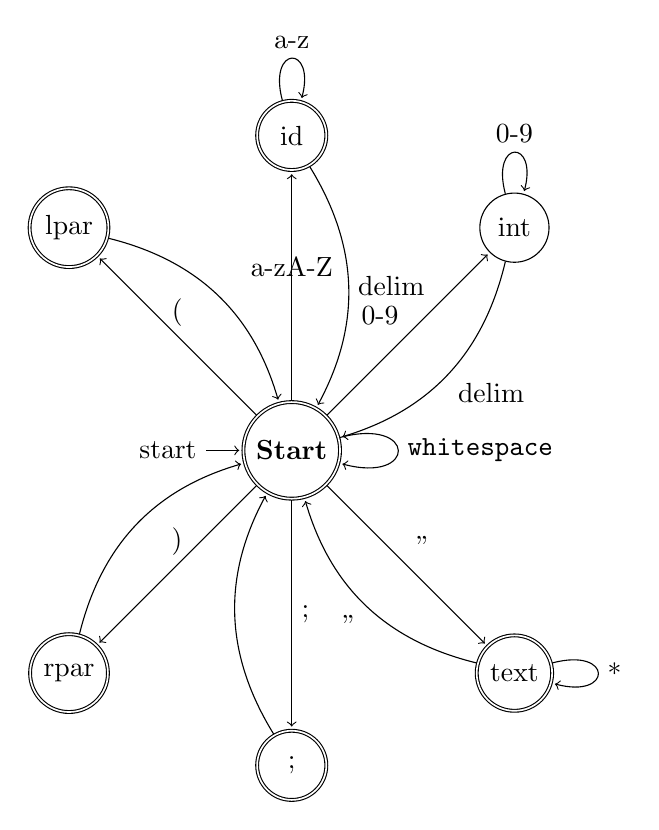
\begin{tikzpicture}[shorten >=1pt,node distance=4cm,on grid,auto] 
   \node[state,initial,accepting] (start)   {\textbf{Start}}; 
   \node[state] (int) [above right=of start] {int}; 
   \node[state,accepting] (text) [below right=of start] {text}; 
   \node[state,accepting](lpar) [above left=of start] {lpar};
   \node[state,accepting](id) [above=of start] {id};
   \node[state,accepting] (rpar) [below left=of start] {rpar};
   \node[state,accepting] (semicolon) [below=of start] {;};
   \path[->] 
   	(start) edge node {0-9} (int)
    		edge node[above] {a-zA-Z} (id)
		edge node[above]  {(} (lpar)
		edge node[above] {)} (rpar)
		edge node{;} (semicolon)
		edge node {"} (text)
		edge [loop right]node {$\mathtt{whitespace}$} ()
		
		(lpar) edge [bend left] node {} (start)
		(rpar) edge [bend left] node {} (start)		
		(semicolon) edge [bend left] node {} (start)
		(id) edge [loop above] node {a-z} ()
			edge [bend left] node {delim} (start)
		(int) edge [loop above] node {0-9} ()
			edge [bend left] node {delim} (start)			
		(text) edge [bend left] node {"} (start)
			edge [loop right] node {*} ()
    ;
\end{tikzpicture}
\end{widetext}

As shown in the diagram, {start}
is the main entry point, from there the immediate possible states, depending
on leading significant character, are {integer}, {identifier}, {keyword}
(static identifiers), {text} (string) and {singleToken}. Using function pointer
the {error} state doesn't need to be specified, instead the function pointer
will be set to nil, so the lexing will terminate.

There are details omitted in this diagram, mainly due to space constraints, such
as escaping with character {\large \texttildelow}, the definition of ``delim'' including
whitespace and state transition leading characters.

\subsection{Emit Tokens}

Upon successful lexing a token, the lexer emits this token to its message
channel, this channel can be consumed by a potential parser, a logging / print
mechanism or any interested party. One obvious feature of this implementation
is that the parsing and lexing can be run at the same time.

\subsubsection{Token Type}
Our Lexer deals with a language that has these token types:

\begin{table}[h]
\centering
\begin{tabular}{l|l}
$\mathbf{Type}$& Description \\
\hline
$\mathtt{id}$& identifiers \\
$\mathtt{int}$& integers \\
$\mathtt{lpar}$& left parenthesis \\
$\mathtt{rpar}$& right parenthesis \\
$\mathtt{semicolon}$& ;s \\
$\mathtt{string}$& strings \\
$\mathtt{error}$& errors
\end{tabular}
\end{table}

With whitespace characters deemed as natural delimiters, and at cases the
transition between $\mathtt{<id>}$ and $\mathtt{<int>}$ is also deemed as delimiter. The $\mathtt{<lpar>}$,
$\mathtt{<rpar>}$ and $\mathtt{<semicolon>}$ are both delimiter and tokens.
The error token will effectively terminate consumption from client.

\subsection{Lexing Integers}

To avoid overflowing the parsing of input integer is performed character by character, such that as soon as already parsed number threatens the exceeding of \textit{max\_int} by either advancing by 10 fold, or with the addition of next digit, the parsing will ignore further digits and return -1. This avoids the pitfall of overflowing integer should the input integer string is too large.\ref{lex-integer}
\begin{widetext}
\begin{lstlisting}[label=lex-integer,caption=lexInteger]
var rst int
const maxint = 65535
for {
	r := l.Next()
	if r == EOF {
		break
	}
	if i := int(r - '0'); i >= 0 && i <= 9 {
		if rst <= 6553 && rst > -1 {
			rst *= 10
			if maxint-rst < i {
				rst = -1
			} else {
				rst += i
			}
		} else {
			rst = -1
			// not break, instead skip until transition
		}
	} else {
		// potentially a state transition here
		l.Backup()
		break
	}
}	
\end{lstlisting}
\end{widetext}

\subsection{Escaping special character}
The target language defined tilde $\thicksim$ as escape character. To realize the escape logic, an efficient way is to use a second pointer and output the extra escaped string in the same pass.

\section{Flex}
Implementing the same lexer using flex is very similar to the Go implementation but much simpler in some aspects. In fact I ported the Go implementation directly to C with virtually no syntax modification. The difference and difficulty of writing flex rules is to adhere to its state matching ordering logic. Because of flex's \texttt{regex} parsing is from top to down, some backtracking logic must be expressed using state or condition, for example the matching of EOF while trying to find the end quote must be put in front of the string rule (for the un-matched the string object to fallback to).

\section{Test and benchmark results}
Writing good tests is both important quality benchmark and tremendous helper for implementing design using language such as Go: it's a good mix of both top down and bottom up practice, and couples with Go's expressiveness one can write complex programs without a debugger. Thanks to the testing facilities available as standard library, testing and benchmarking is very straight-forward. Even automatically generating complex profiling diagrams would not require much more effort.
While all test and benchmark results are attached in appendix, I would like briefly give an overview of those in this section.

\subsection{Test result for Go Lexer and Flex}
The input examples are provided by lecturer, originally labeled as \textbf{input[1-9].txt}. Both Go Lexer and Flex are tested against these example inputs. Further there are few unit tests for Go implementation, all Go tests are to be found in source code listing labeled with \textbf{xxx\_test.go}
The Go test result are embodied with simple benchmark timer and heading indicating individual test methods and its result, therefore it's more verbose. Readers should seek to heading after \textbf{TestOutput} to examine the result. The Flex result is just a simple heading followed by result. The format is different but the content is easily comparable.

\subsection{Performance Benchmark and Profiling the Lexer}
With the help of Go testing framework I performed benchmark on both\textbf{(*SymbolTable).Process} and \textbf{(*Lexer).Run}, with short and long sequence test-cases. While due to time constraints I don't have enough data to do vertical comparison between the Go implementation and an proper C implementation, the dumbed version of the C code however did finished processing 37 million words under 11 seconds. Further CPU profiling \footnote{due to the need of archiving certain degree of automation I chose to use buffered IO to read input into memory instead of reading off pipe as stream, there is some extra overhead in terms of loading time.} shows that while \textbf{(*Lexer).Run} occupies roughly 40\% of the CPU time, the major cumulative processing landed in channel communications. 

\section{Appendix Overview}
\begin{enumerate}[$\surd$]
	\item generated code documentation
	\begin{enumerate}[$\blacktriangleright$]
	\item compiler.pdf	
	\end{enumerate}
	\item source code listing: Go Compiler 
	\begin{enumerate}[$\blacktriangleright$]
	\item trie.go; trie\_test.go
	\item lex.go; lex\_test.go
	\item tests.go; doc.go
	\end{enumerate}
	\item source code listing: flex
	\begin{enumerate}[$\blacktriangleright$]
	\item compiler.flex
	\item symboltable.h
	\end{enumerate}
	\item test result / output
	\begin{enumerate}[$\blacktriangleright$]
	\item lexer\_out.pdf
	\item flex\_out.pdf
	\end{enumerate}
	\item benchmarks
	\begin{enumerate}[$\blacktriangleright$]
	\item bench\_go.pdf
	\item cpu-long-profile.pdf
	\end{enumerate}
\end{enumerate}

\rule{\textwidth}{2pt}

\end{document}
%
% ****** End of file aipsamp.tex ******
